
\subsubsection{Карта рассеяния в прямом пространстве}

\begin{figure}[H]
  \centering
  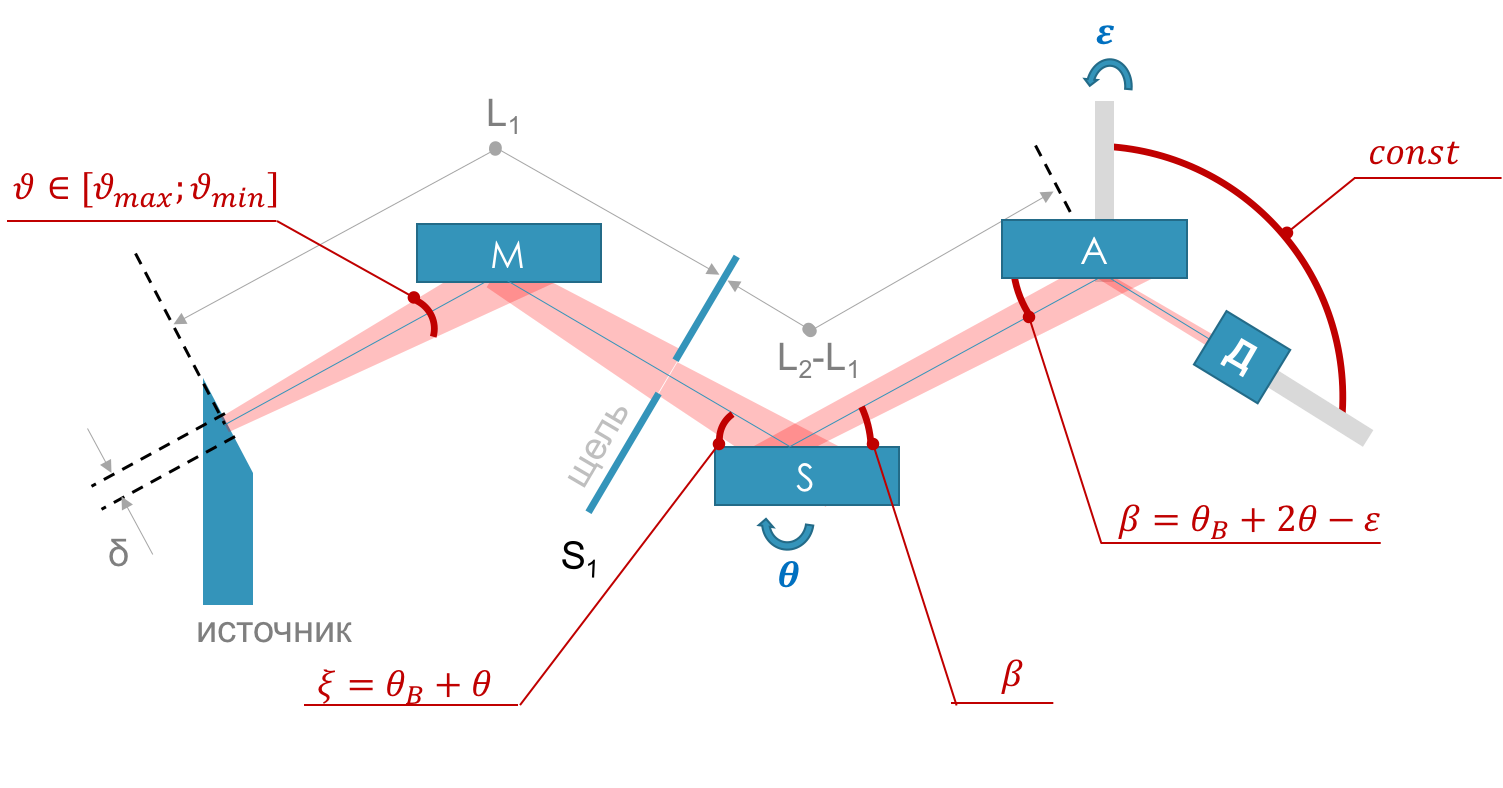
\includegraphics[width=0.8\textwidth]{images/triple_crystal_schem.png}
  \caption{Схема трехкристального эксперимента, $\theta$ - отстройка образца от точного угла Брегга,
  $\epsilon$ - угол анализатора относительно зеркально отраженного пучка образцом}
  \label{ris:}
\end{figure}

\begin{eqnarray} \label{eq:doudle_spectra_angle_map}
  P_{triple}(\theta,\varepsilon) = \sum_{\lambda = -\infty}^{\infty}g_{\lambda}(\lambda)\cdot
  \sum_{\vartheta = \vartheta_{s1}}^{\vartheta_{s2}} \Bigg[ g_{\vartheta}(\vartheta) g_{S}(\vartheta) \cdot \nonumber \\
    P_M \left(\vartheta - \frac{\lambda - \lambda_1}{\lambda_1}\tan(\theta_B) \right) \cdot \nonumber \\
   P_S \left(\theta + \vartheta - \frac{\lambda - \lambda_1}{\lambda_1}\tan(\theta_B)\right)  \cdot  \nonumber \\
   P_A \left(2\theta - \varepsilon + \vartheta - \frac{\lambda - \lambda_1}{\lambda_1}\tan(\theta_B)\right) \Bigg]
 \end{eqnarray}
